\chapter{Gertaerak eta gertaera-kudeatzaileak}

Web orri baten barruko elementuen egoera aldatzean, gertaerak altxatzen dira. Adibidez, botoi baten gainean klik egitean, botoiaren egoera aldatu dela adierazteko, nabigatzaileak gertaera bat altxatuko du \index{onclick}(\textit{onclick} gertaera, hain zuzen ere). Edo orri baten elementu guztiak kargatzen bukatzean, \index{onload}\textit{onload} gertaera altxatuko da. Gertaerak tratatu nahi izanez gero, gertaera-kudeatzaile bat programatu beharko dugu. Ezezkoan, ez dugu ezer egin behar, alegia, gertaera altxatuko da, baina ez badu inork tratatzen, ez da ezer gertatuko.


\section{Gertaera motak}

Adibideetan ikusi dugun bezala, bi gertaera mota daude: erabiltzaileak sortutakoak (botoi baten gainean klik egin, sagua mugitu, leihoa handitu, tekla bat sakatu...) eta sistemak automatikoki sortutakoak (orri baten elementuak kargatzen bukatzean, bideo bat bistaratzeko prest dagoenean, errore bat gertatzen denean...).  Azter ditzagun horrelako gertaera zehatzen adibide batzuk.

\subsection{Erabiltzaileak sortutako gertaerak}

Maiz erabiltzen diren gertaera mota hauen adibideak:
\begin{itemize}
\item onclick (saguarekin elementu baten gainean klik egitean)
\item \index{onmouseover} onmouseover (sagua elementu baten gainean jartzean)
\item \index{onblur} onblur (elementu batek fokua galtzen duenean)
\item \index{onfocus} onfocus (elementu batek fokua hartzen duenean)
\item \index{ondrag} ondrag (elementu bat arrastatzean)
\item \index{onkeypress} onkeypress (tekla bat sakatzean)
\end{itemize}


\subsection{Sistemak sortutakoak}
  Maiz erabiltzen diren gertaera mota hauen adibideak:

\begin{itemize}
\item \index{onload} onload (elementu bat kargatzen bukatzean)
\item \index{oncanplay} oncanplay (elementu multimedia bat kargatu eta ikusi edo jo dezakegunean)
\item \index{onoffline} onoffline (konexioa galtzean)
\end{itemize}


\section{Nola kudeatu gertaerak JavaScript-en}

Hiru modu ezberdin daude gertaerak JSn kudeatzeko. Kudeatzaileak HTML kodean txertatuz, gertaeraren iturri-osagaiaren gainean kudeatzaile bat zuzenean definituz edo \index{addEventListener} metodo generikoa erabiliz.

\subsubsection{JavaScript HTML kodean txertatu}

Elementuaren ostean \textit{onclik} atributuan zer funtzio exekutatu nahi dugun zehaztuko dugu, adibidez:

\begin{lstlisting}[language=JavaScript,numbers=none]
<button onclick="alert('Hello world');">
  Sakatu hemen
</button>
\end{lstlisting}

\subsubsection{Osagaiaren gainean kudeatzailea zuzenean definitu}

Askotan gomendagarria da gertaera-kudeatzaileak JS fitxategi batean gordetzea eta funtzio horiek osagaiaren izena erabiliz zehaztea, honelako patroiari jarraituz:

\begin{lstlisting}[language=JavaScript,numbers=none]
osagaia.gertaera = function()
{
   // gertaera kudeatzeko kodea
}
\end{lstlisting}

Adibidez, aurreko adibide bera honela programatu dezakegu:
\begin{lstlisting}[language=JavaScript,numbers=none]
  botoia.onclick = function()
  {
    //
   // gertaera kudeatzeko kodea
   };
\end{lstlisting}

\index{addEventListener}
\subsubsection{addEventListener metodo generikoa erabiliz}

\textit{addEventListener} metodoak 2 parametro hartzen ditu\footnote{addEventListener metodoa gainkargatuta dago, alegia, 2 parametro baino gehiagoko bertsioak ere baditu. addEventListener eta removeEventListener inguruan informazio gehiago MDNn aurkituko duzu (\href{https://developer.mozilla.org/en-US/docs/Web/API/EventTarget/addEventListener}{https://developer.mozilla.org/en-US/docs/Web/API/EventTarget/addEventListener}).}, tratatu nahi dugun gertaeraren izena eta funtzio-kudeatzailearen izena, eskema honi jarraituz:

\begin{lstlisting}[language=JavaScript,numbers=none]
osagaia.addEventListener('gertaera', funtzioa);
\end{lstlisting}

Gauza bera gertaera-kudeatzaile bat elementu batetik ezabatu nahi izanez gero. Kasu honetan, \textit{removeEventListener} metodoa erabiliko dugu.

Adibidez, botoiaren gainean sakatzean funtzio bat exekutatzeko:

\begin{lstlisting}[language=JavaScript,numbers=none]
botoia.addEventListener('click', funtzioarenizena);
\end{lstlisting}

Eta momentu batean esleipen hori kendu nahiko bagenu, \index{removeEventListener}\textit{removeEventListener} erabiliko genuke:

\begin{lstlisting}[language=JavaScript,numbers=none]
botoia.removeEventListener('click', funtzioarenizena);
\end{lstlisting}


\section{Adibide praktikoa}

Demagun \ref{fig:gertaerakadibidepraktikoa}. irudian ikusten den bezalako webgune bat dugula. Irudian zenbait errezetaren argazkiak agertuko dira, sekuentzian. Gure helburua errezeta baten gainean klik egitean, kontsolan mezu bat agertzea da.

\begin{figure}[ht]
	\centering
\begin{tikzpicture}
\node[anchor=south west,inner sep=0] (image) at (0,0)
   {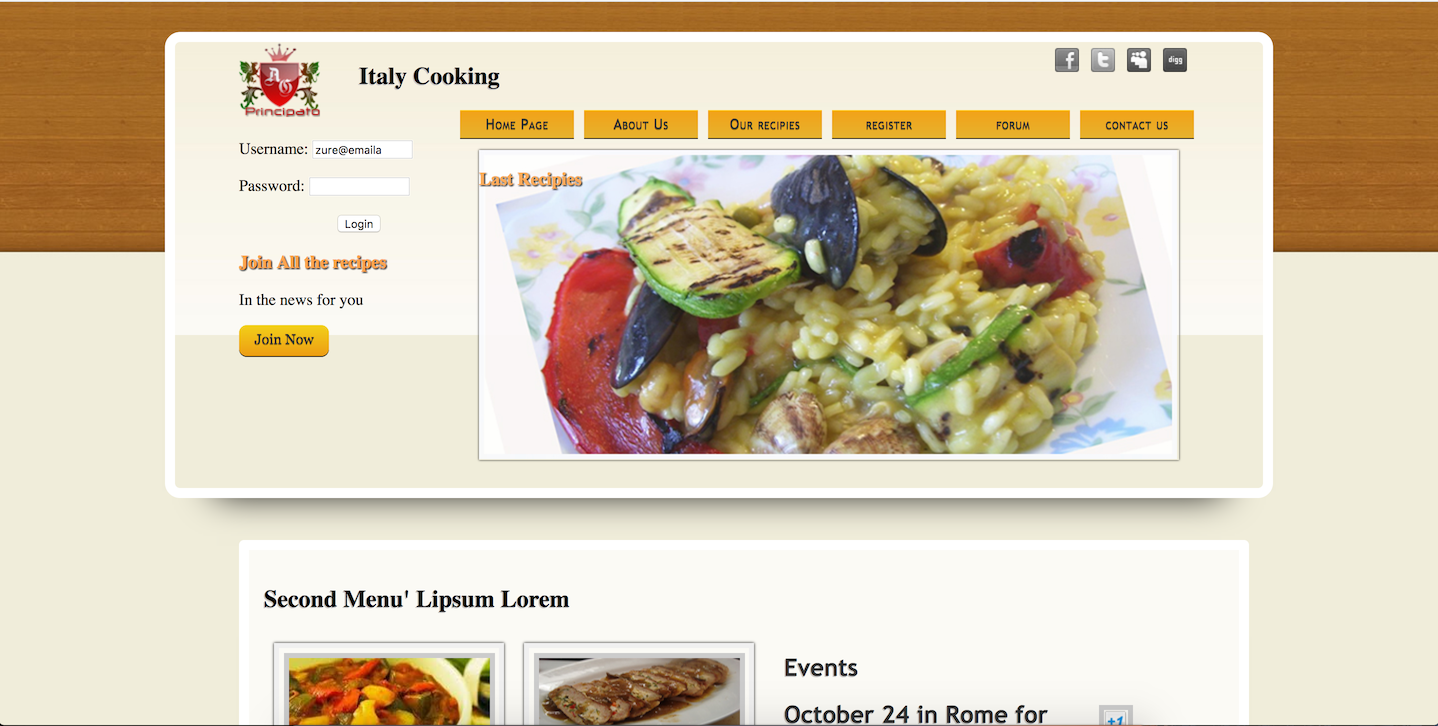
\includegraphics[trim=0cm 0cm 0cm 0cm, clip=true, width=0.75\textwidth]{img/errezetak}};
\end{tikzpicture}
\caption{Gertaerak: adibide praktikoak.}
\label{fig:gertaerakadibidepraktikoa}
\end{figure}




\begin{lstlisting}[language=JavaScript,numbers=none]
function kudeatzaileakHasieratu()
{
   let irudia = document.getElementById('irudia');
   irudia.onclick = function() {
      console.log("Irudia sakatu duzu");
  }
}


window.onload = kudeatzaileakHasieratu;
\end{lstlisting}

\index{onload}
Garrantzitsua da \textit{window.onload}-en gertaera-kudeatzailea zehaztea. Horrela egingo ez bagenu, eta zuzenean \hl{kudeatzaileakHasieratu} metodoari deituko bagenio,
posible litzateke irudia oraindik kargatu gabe egotea, eta, hortaz, \hl{getElementById()} egitean \textit{null} aurkitzea.

\subsubsection{Gertaerak kudeatzen: \textit{onblur}, \textit{onfocus}}

Aurreko irudian ikusten dugun inprimakian erabiltzailearen datuak (email-helbide eta pasahitza) eskatzen dira. Helbide elektroniko bat testu-eremu batean idatzi behar duela gogorarazteko trikimailu bat erabil dezakegu \textit{onblur} gertaeraz baliatuz. Erabiltzaileak email-helbidea ez badu oraindik idatzi eta horretarako dagoen testu-eremua hutsik badago, orduan \textquotedbl{}zure@emaila\textquotedbl{} bezalako argibidea idatziko dugu bertan testu-eremu horrek fokua galtzean (\textit{onblur}). Berriz, testu-eremu horrek berriro fokua hartzen duenean (\textit{onfocus}), eta oraindik email-helbidea idatzi gabe badu, balioa hustu egingo dugu. 

\begin{lstlisting}[language=JavaScript]
let erabiltzaile = document.getElementById('erabiltzaile');
erabiltzaile.value = 'zure@emaila';

erabiltzaile.onfocus = function(event){
  let input = event.target
  if (input.value == 'zure@emaila'){
    erabiltzaile.value = '';
 }
}

erabiltzaile.onblur = function(event){
	let input = event.target
	if (input.value == ''){
	    erabiltzaile.value = 'zure@emaila';
  	}
}

\end{lstlisting}

\subsubsection{Gertaerak kudeatzen: \textit{onchange}}

Erabiltzaileak aukera-zerrenda (\textit{combobox}) bateko aukeraren bat hautatzean \textit{onchange} gertaera altxatzen da. Zerrendan hainbat osagai daude <select> etiketaren  barruan:

\begin{lstlisting}[language=HTML,numbers=none]
    <option value="rice">Arroza</option>
    <option value="mushrooms">Txanpinoiak</option>
\end{lstlisting}

Hurrengo adibidean \textit{zerrendaKudeatzaile} funtzio bat prestatu dugu gertaera horri erantzuteko. Zehazki, aukeratu den elementuaren balioa (\textit{value} atributuan dagoena), elementu horren indizea zerrendan \index{\textit{selectedIndex}}(selectedIndex) eta aukera horren testua (adibidez, Arroza).

\begin{lstlisting}[language=HTML5]
let item = document.getElementById('combobox');
item.addEventListener('change', zerrendaKudeatzaile);

function zerrendaKudeatzaile(event){
   let item = event.target
   console.log(item.value); // rice
   console.log(item.selectedIndex);  // 2
   console.log(item.options[item.selectedIndex].text); // Rice with mushrooms
}

<select name="GoMenu" style="width:159px" id="combobox">
<option selected="selected">Select a recipe</option>
<option class="_self" value="spaghetti">Spaghetti with aubergine</option>
<option class="_self" value="rice">Rice with mushrooms</option>
<option class="_self" value="rolls">Rolls with polenta</option>
<option class="_self" value="chicken">Chicken Hunter</option>
<option class="_self" value="tortiglioni">Tortiglioni filled</option>
<option class="_self" value="swordfish">Smoked swordfish</option>
<option class="_self" value="pumpkins">Stuffed pumpkins</option>
</select>
\end{lstlisting}

\subsubsection{Gertaerak kudeatzen: \textit{onsubmit}}
Inprimaki baten \textit{onsubmit} gertaera inprimakiaren ``Bidali'' botoian sakatzean altxatzen da. Gertaera hori erabil dezakegu inprimakian sartu diren balioak zuzenak diren edo ez egiaztatzeko (zerbitzarira bidali baino lehen). Horretarako, funtzio bat esleituko diogu \textit{onsubmit} kudeatzaileari. Funtzio horrek parametroak aztertu eta denak zuzenak badira, \hl{true} bueltatu behar du. \hl{False} kontrako kasuan.

\begin{lstlisting}[language=JavaScript]
let inprimakia = document.getElementById('inprimakia');
inprimakia.onsubmit = function(){
console.log("Bidali botoian klikatu duzu");
 // eremuak baliostatu. 
// Baten bat bete gabe balego, false itzuli
// Bestela, true itzuli
return false;
}
\end{lstlisting}

\subsubsection{Gertaerak kudeatzen: \textit{onchange} \textit{range}}

\index{range}
Inprimaki baten \textit{range} motako osagaiak \textit{onchange} gertaera altxatzen du erabiltzaileak tiraderatik tira egiten duenean alde batera edo bestera. \textit{Range} osagaiaren balioa une oro ikusi ahal izateko, gertaera horri honako kudeatzailea esleitu diezaiokegu:

\begin{lstlisting}[language=JavaScript]
<form>
 <input type='range' min=1 max=100 step=1 id='tartea'>
 </form>

 <div id='balioa'></div>
 <script>
let kudeatzaileHasieratu = function()
{
   let tartea = document.getElementById('tartea');
   tartea.addEventListener('change', balioaBistaratu)

   function balioaBistaratu( event ){
       let tartea = event.target
       document.getElementById('balioa').innerHTML = tartea.value;
   }
} 

window.onload = kudeatzaileaHasieratu;
</script>

\end{lstlisting}

\subsubsection{Gertaerak kudeatzen: \textit{setTimeout}, \textit{setInterval}}

\index{setTimeout}
\index{setInterval}
Bukatzeko, aldiro-aldiro funtzio bat exekutatu nahiko bagenu (adibidez, 5 segundoan behin funtzio bat exekutatu nahiko bagenu), oso interesgarria litzateke \textit{setInterval} metodoa. Bi parametro hartzen ditu, exekutatu nahi den funtzioaren izena eta zer maiztasunez exekutatu nahi dugun, milisegundotan.

Adibidez, idatzi() izeneko funtzioa 5 segundoan behin exekutatu nahiko bagenu:
\begin{lstlisting}[language=JavaScript]
function idatzi() {
       console.log("Idazten..." + new Date());
}
let erlojua = setInterval(idatzi, 5000);
\end{lstlisting}

Beste batzuetan ez dugu aldiro-aldiro exekutatu nahiko, baizik eta behin bakarrik X segundo pasa ostean. Horretarako, \textit{setTimeOut} funtzioa erabiliko dugu. Adibidez, idatzi funtzioa 5 segundo barru exekutatzeko (ez aldiro, baizik eta soilik behin, 5 segundo barru):

\begin{minipage}{\linewidth}
\begin{lstlisting}[language=JavaScript]
function idatzi()
{
      console.log("Idazten...." + new Date());
}
let reloj = setTimeOut(idatzi, 5000);
\end{lstlisting}
\end{minipage}

\section{Ariketak}

Gai honen inguruan planteatzen diren ariketak webgune baten gainean egin behar dira. Jaitsi beharrezkoak diren txantiloia \href{https://www.ikasten.io/html5/ariketak/fitxategiak/06_txantiloia.zip}{https://labur.eus/2DWcm} (ikasten.io) eta  irudiak \href{https://www.ikasten.io/html5/ariketak/fitxategiak/06_irudiak.zip}{https://labur.eus/BiAms} (ikasten.io) eta jarrai iezaiezu ariketa egiteko argibideei.

\begin{itemize}
    \item JavaScript erabiliz dinamikoki alda daiteke <div> etiketa baten barruan zehazten den irudia. Adibidez, \ref{fig:gertaerak-ariketa-1}. irudian dugun webgunearen kasuan, errezetaren irudia alda dezakegu.
    
    \begin{figure}[ht]
	\centering
\begin{tikzpicture}
\node[anchor=south west,inner sep=0] (image) at (0,0)
   {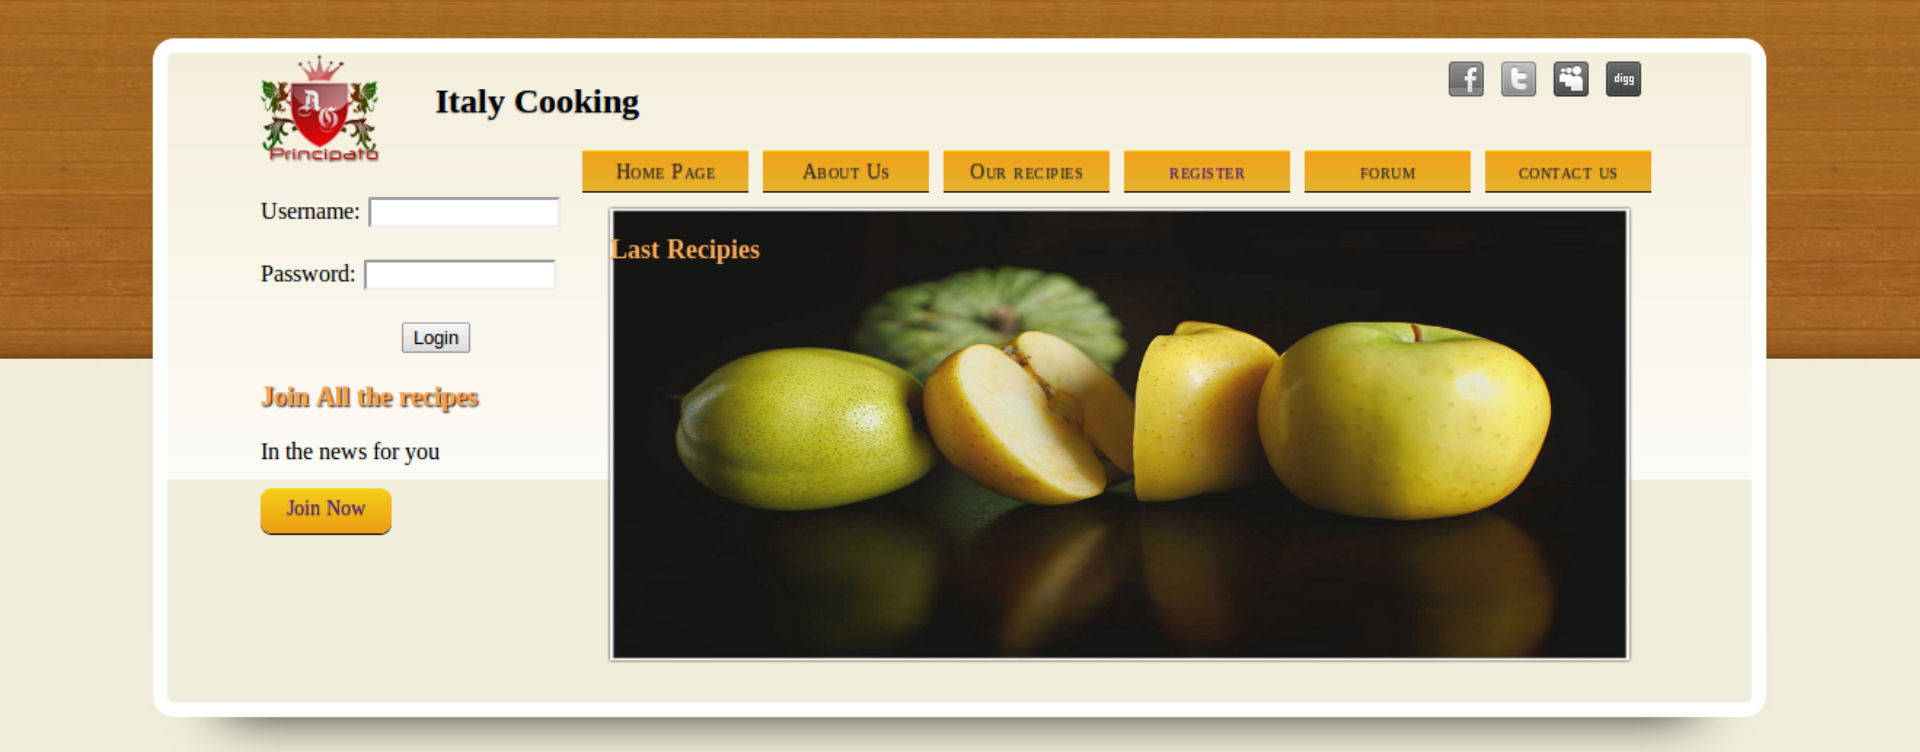
\includegraphics[trim=0cm 0cm 0cm 0cm, clip=true, width=0.75\textwidth]{img/gertaerak/gertaerak_ariketa_2.png}};
\end{tikzpicture}
\caption{Gertaerak: ariketaren hasierako egoera.}
\label{fig:gertaerak-ariketa-1}
\end{figure}

Horretarako, honako kodea erabiliko dugu:

\begin{lstlisting}[language=JavaScript,numbers=none]
let irudia = document.getElementById("irudia")
irudia.style.backgroundImage = "url(irudiak/irudiberria.jpg)"
\end{lstlisting}

Ariketa honetan irudi hori 5 segundoan behin aldatzea  eskatzen da (ikus \ref{fig:gertaerak-ariketa-2}. irudia). Sei irudiz osatutako array batetik hartuko dugu hurrengo irudia. Alegia, gai honetan ikusi dugun webgunean oinarrituta, beharrezkoa den JavaScript kodea programatu irudi guztiak sekuentzian bistaratzeko (5 segundoan behin). Erabiltzaileak irudiaren gainean sakatzen badu, irudien animazioa eten egin behar da. Irudiaren gainean ez badu sakatzen, 6. irudiaren ondoren berriro lehenengoa bistaratuko da, sekuentziari jarraituz (ikus: \href{http://www.youtube.com/watch?v=aaoNMmnfGD4}{http://www.youtube.com/watch?v=aaoNMmnfGD4}).

\begin{figure}[ht]
	\centering
\begin{tikzpicture}
\node[anchor=south west,inner sep=0] (image) at (0,0)
   {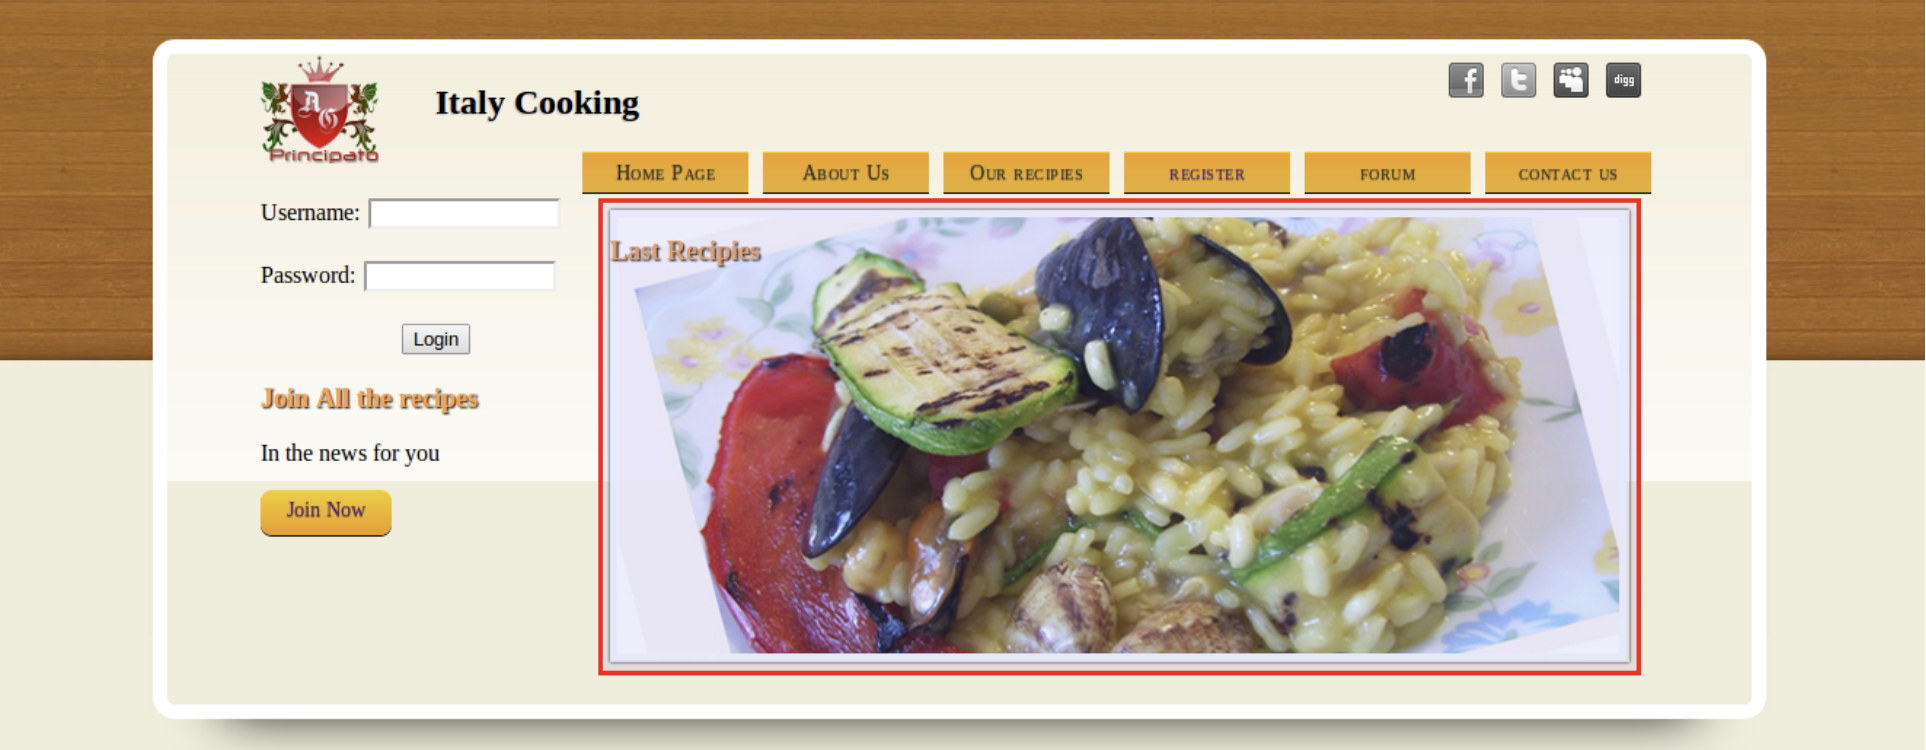
\includegraphics[trim=0cm 0cm 0cm 0cm, clip=true, width=0.75\textwidth]{img/gertaerak/gertaerak_ariketa_1.png}};
\end{tikzpicture}
\caption{Gertaerak: ariketaren helburu-egoera.}
\label{fig:gertaerak-ariketa-2}
\end{figure}




\end{itemize}
